% Options for packages loaded elsewhere
\PassOptionsToPackage{unicode}{hyperref}
\PassOptionsToPackage{hyphens}{url}
\PassOptionsToPackage{dvipsnames,svgnames*,x11names*}{xcolor}
%
\documentclass[
  11pt,
]{article}
\usepackage[]{mathpazo}
\usepackage{amsmath}
\usepackage{ifxetex,ifluatex}
\ifnum 0\ifxetex 1\fi\ifluatex 1\fi=0 % if pdftex
  \usepackage[T1]{fontenc}
  \usepackage[utf8]{inputenc}
  \usepackage{textcomp} % provide euro and other symbols
  \usepackage{amssymb}
\else % if luatex or xetex
  \usepackage{unicode-math}
  \defaultfontfeatures{Scale=MatchLowercase}
  \defaultfontfeatures[\rmfamily]{Ligatures=TeX,Scale=1}
\fi
% Use upquote if available, for straight quotes in verbatim environments
\IfFileExists{upquote.sty}{\usepackage{upquote}}{}
\IfFileExists{microtype.sty}{% use microtype if available
  \usepackage[]{microtype}
  \UseMicrotypeSet[protrusion]{basicmath} % disable protrusion for tt fonts
}{}
\makeatletter
\@ifundefined{KOMAClassName}{% if non-KOMA class
  \IfFileExists{parskip.sty}{%
    \usepackage{parskip}
  }{% else
    \setlength{\parindent}{0pt}
    \setlength{\parskip}{6pt plus 2pt minus 1pt}}
}{% if KOMA class
  \KOMAoptions{parskip=half}}
\makeatother
\usepackage{xcolor}
\IfFileExists{xurl.sty}{\usepackage{xurl}}{} % add URL line breaks if available
\IfFileExists{bookmark.sty}{\usepackage{bookmark}}{\usepackage{hyperref}}
\hypersetup{
  colorlinks=true,
  linkcolor=Maroon,
  filecolor=Maroon,
  citecolor=Blue,
  urlcolor=blue,
  pdfcreator={LaTeX via pandoc}}
\urlstyle{same} % disable monospaced font for URLs
\usepackage[margin=1in]{geometry}
\usepackage{graphicx}
\makeatletter
\def\maxwidth{\ifdim\Gin@nat@width>\linewidth\linewidth\else\Gin@nat@width\fi}
\def\maxheight{\ifdim\Gin@nat@height>\textheight\textheight\else\Gin@nat@height\fi}
\makeatother
% Scale images if necessary, so that they will not overflow the page
% margins by default, and it is still possible to overwrite the defaults
% using explicit options in \includegraphics[width, height, ...]{}
\setkeys{Gin}{width=\maxwidth,height=\maxheight,keepaspectratio}
% Set default figure placement to htbp
\makeatletter
\def\fps@figure{htbp}
\makeatother
\setlength{\emergencystretch}{3em} % prevent overfull lines
\providecommand{\tightlist}{%
  \setlength{\itemsep}{0pt}\setlength{\parskip}{0pt}}
\setcounter{secnumdepth}{-\maxdimen} % remove section numbering
\usepackage{booktabs}
\usepackage{xcolor}
\usepackage{booktabs}
\usepackage{longtable}
\usepackage{array}
\usepackage{multirow}
\usepackage{wrapfig}
\usepackage{float}
\usepackage{colortbl}
\usepackage{pdflscape}
\usepackage{tabu}
\usepackage{threeparttable}
\usepackage{threeparttablex}
\usepackage[normalem]{ulem}
\usepackage{makecell}
\usepackage{xcolor}
\ifluatex
  \usepackage{selnolig}  % disable illegal ligatures
\fi

\title{Comparative Politics\footnote{This syllabus is heavily inspired
  by similar courses by \href{https://graemeblair.com/}{Graeme Blair},
  \href{https://virginiaoliveros.com/}{Virginia Oliveros}, and
  \href{http://yujeongyang.weebly.com/}{Yujeong Yang}.}\\
POLC 2300-01 (3 credits)\\
Fall 2021\\
Tuesdays and Thursdays, 9:30 - 10:45 AM\\
118 Norman Mayer Building}
\author{}
\date{\vspace{-2.5em}}

\begin{document}
\maketitle

\textbf{Instructor:} Gustavo Diaz\\
\textbf{Office location:} Center for Inter-American Policy and Research,
7025 Freret St, First floor\\
\textbf{Office hours:} Tuesdays and Thursdays, 11AM - 12PM or by
appointment (virtual preferred)\\
\textbf{Email address:}
\href{mailto:gustavodiaz@tulane.edu}{\nolinkurl{gustavodiaz@tulane.edu}}

\hypertarget{course-description}{%
\section{Course Description}\label{course-description}}

This course offers an introduction to comparative politics. Comparative
politics is the subfield of Political Science that tries to understand
variation in political institutions, political behavior, public
policies, and their outcomes.

The course focuses on building the analytical tools to understand
comparative politics, as well as the central questions in the subfield.
These central questions include:

\begin{enumerate}
\def\labelenumi{\arabic{enumi}.}
\tightlist
\item
  How do democracies rise and fall?
\item
  How do regime types affect types affect the economic and political
  performance of a country?
\item
  How do institutional arrangements vary within and across regime types?
\item
  How do these institutional arrangements affect economic and political
  outcomes?
\end{enumerate}

We start with a discussion of the origins of comparative politics and
its current role within Political Science. Then, we explore the origins
of nation-states, governments, and regime types. From there, we address
the causes and consequences of different regime types, including
variation within democracies and autocracies.

\hypertarget{course-goals}{%
\section{Course Goals}\label{course-goals}}

This course has three goals:

\begin{enumerate}
\def\labelenumi{\arabic{enumi}.}
\item
  Familiarize students with the study of comparative politics
\item
  Build core analytical skills central to the study of politics around
  the world
\item
  Strengthen communication skills by learning and practicing concepts
  from comparative politics
\end{enumerate}

\hypertarget{course-learning-objectives}{%
\section{Course Learning Objectives}\label{course-learning-objectives}}

By the end of the course, we will be able to:

\begin{enumerate}
\def\labelenumi{\arabic{enumi}.}
\item
  Understand the fundamentals of comparative politics
\item
  Engage in productive conversations on politics and policy around the
  world
\item
  Apply the analytical skills from the course to our current and future
  careers
\end{enumerate}

\hypertarget{required-student-resources}{%
\section{Required Student Resources}\label{required-student-resources}}

\hypertarget{prerequisites}{%
\subsection{Prerequisites}\label{prerequisites}}

There are no formal prerequisites to take this course.

\hypertarget{technology}{%
\subsection{Technology}\label{technology}}

You will need reliable access to a computer with internet connection to
access the course material and to work on and submit assignments. We
will use Canvas as a hub for all course related purposes. Please let me
know if you need help accessing technology resources.

\hypertarget{reading}{%
\subsection{Reading}\label{reading}}

We will use the following textbook:

\begin{itemize}
\tightlist
\item
  Clark, William Roberts, Matt Golder, and Sona N. Golder. 2017.
  \emph{Principles of Comparative Politics}. Washington DC: CQ Press.
  Third Edition.
  \href{https://tulane.bncollege.com/shop/BNCB_TextbookDetailView?displayStoreId=13559\&urlRequestType=Base\&catalogId=10001\&productId=600007976346\&langId=-1\&partNumber=MBS_1944592\&storeId=13559\&sectionId=102216419\&item=N}{\texttt{{[}TU\ Bookstore{]}}}
  \href{https://www.amazon.com/Principles-Comparative-Politics-William-Roberts/dp/1506318126}{\texttt{{[}Amazon{]}}}
\end{itemize}

The rest of the syllabus refers to the textbook as CGG. We will use the
third edition. The second edition may also work, with the exception of
the chapters listed \href{http://mattgolder.com/books/pocp}{here}. Don't
bother with the international edition.

I will also list recommended readings in the course schedule. I may
mention some during class, but I do not expect you to read them. They
are mostly for your future reference.

Also for your reference, you can see the list of comparative politics
courses that you may take after this introductory course
\href{https://catalog.tulane.edu/courses/polc/}{here}.

\hypertarget{evaluation-procedures-and-grading-criteria}{%
\section{Evaluation Procedures and Grading
Criteria}\label{evaluation-procedures-and-grading-criteria}}

Your grade will depend on the following assignments:

\begin{table}[!h]
\centering
\begin{tabular}[t]{ll}
\toprule
Assignment & Percentage\\
\midrule
\cellcolor{gray!6}{Quizzes (6)} & \cellcolor{gray!6}{40\%}\\
News Reports (6) & 40\%\\
\cellcolor{gray!6}{Participation} & \cellcolor{gray!6}{20\%}\\
Final Exam & 30\% of final grade\\
\bottomrule
\end{tabular}
\end{table}

\hypertarget{quizzes-40}{%
\subsection{Quizzes (40\%)}\label{quizzes-40}}

We will have six online quizzes every other week. These are a
combination of selection and short answer questions including material
from the textbook and lectures. Every quiz will cover the material
discussed after the last quiz.

Quizzes become available on Canvas on Thursdays at noon CT and are due
on Fridays of the same week by 5pm CT. Each quiz is worth 10 points and
only your best five quizzes count towards your final grade.

\hypertarget{news-reports-40}{%
\subsection{News reports (40\%)}\label{news-reports-40}}

On the weeks without Quizzes (except for weeks 1 and 13), you will
submit a news report covering recent political events in a region of the
world of your choosing. I encourage you to be creative about the meaning
of ``political'' and ``region.'' The purpose of news reports is to apply
the course material to current world events and to practice short-form
communication. You will submit six reports in total.

Except for the first report, you can use any creative medium to deliver
your news report. If you write a short essay, your report should be no
longer than two pages (12pt font, double spaced). Some examples of
alternative creative mediums include: audio, video, drawing, painting,
infographics, concept maps, and flowcharts.

My ultimate goal is for you to use the course as an opportunity for
advancing your personal interests and career goals, so the only
restriction is that you choose a medium that can be uploaded or linked
in canvas and that I can reasonably grade within a week. Don't overdo
it! Find something that will be fun and sustainable throughout the
semester.

If your report does not include an equivalent amount of written or
spoken words, you should attach a document no longer than one page
explaining your intention. If your creative medium cannot accommodate a
reference to the sources you use, you should also attach those in a
separate document.

Your first news report will propose a region of the world to follow,
explain why you think it would be interesting to follow the news from
that region, include a list of five potential news sources, and explain
the creative medium that you plan to use. I will discuss news reports in
more detail on week 3. Your choice of region or creative medium is not
binding, but you should consult with me if you plan to change your
original focus.

Every subsequent news report should contain a brief summary of events or
opinions surrounding them, a justification of why these are important
events, and your own thoughts or opinions regarding the events in
question. If any of those aspects is not immediately obvious, you should
clarify it in an attachment. An excellent news report uses the course
material to shed new light on recent events.

News reports are due on the Friday of the week they appear as due in the
course schedule by 5pm CT. You will upload or share a link to your
report using the corresponding space on Canvas. Each report is worth 10
points and only your best five reports count towards your final grade.

\hypertarget{participation-20}{%
\subsection{Participation (20\%)}\label{participation-20}}

I expect you to engage actively in this class. At a minimum, I expect
you to come to lecture ready to discuss the material. To obtain a good
participation grade, you must also make interventions conducive to a
productive and respectful learning environment for yourself and others
during class, office hours, in Canvas, or through other means that best
suit your learning style.

We all have different learning styles, so I will keep an open mind about
what constitutes good participation, and I encourage you to be proactive
about pursuing the participation avenues that are most productive for
you.

You will receive a temporary participation grade during Fall break along
with feedback on how to improve. As a rule of thumb, if I remember your
name, you are likely in the right track. Participation scores range from
0 to 100.

\hypertarget{final-exam-30-of-final-grade}{%
\subsection{Final Exam (30\% of final
grade)}\label{final-exam-30-of-final-grade}}

We will have final exam on the scheduled final examination date for the
course (TBD). The final exam is required only for those without a
passing grade. For everyone else, the final exam is optional.

The final covers the entirety of the course material and uses a format
similar to the quizzes. Your exam will be graded from 0 to 100. If
public health conditions allow, we will hold the final exam in person.

\hypertarget{late-work-policy}{%
\subsection{Late work policy}\label{late-work-policy}}

For each day an assignment is late without excuse, I will deduct 10\% of
your grade for that assignment. If your assignment is late for more than
3 days, your assignment will be graded with zero.

That said, this course is taking place during extraordinary times. If
exceptional circumstances require you to ask for an extension or other
accommodations, reach out to me as soon as possible. If you anticipate
prolonged issues, ask your academic advisor (or equivalent) to send me
an e-mail detailing the extent of required accommodations. For
accessibility or religious accommodations, please read the appropriate
sections below.

Please note that you never owe me personal information about your mental
or physical health, nor about any other aspect of your personal life.
For example, I will not ask for documentation if you need to quarantine
because of a close contact tested positive. However, I do expect you to
be accountable for coursework and reach out if you expect complications
that prevent you from keeping up.

I aim to establish a learning community based on empathy about our
varied circumstances during this time. You are always welcome to talk to
me about what you are going through. I will not judge nor think less of
you, and I hope you will extend me the same courtesy. If I can't help
you, I will help you find the resources on campus that you need.

\hypertarget{grading}{%
\subsection{Grading}\label{grading}}

Final grades range from 0 to 100 and will use the following conversion
to letter grades:

\begin{center}
\includegraphics[width=1\linewidth]{polc2300_syllabus_files/figure-latex/unnamed-chunk-2-1} \end{center}

Final grades with decimal numbers will be truncated to the highest
integer (e.g.~92.1 becomes 93). After this, if your grade is exactly in
the limit between two letter grades, you will get the highest letter
grade (e.g.~93 is an A).

\hypertarget{attendance-statement}{%
\section{Attendance Statement}\label{attendance-statement}}

I do not take attendance, but attendance is a basic component of your
participation grade and some topics may be covered during lecture but
not on the textbook. I trust that you will balance attendance and
participation according to your priorities.

\hypertarget{remote-course-policies}{%
\section{Remote Course Policies}\label{remote-course-policies}}

As long as we are meeting in person, I will not allow remote attendance
unless a formal accessibility request requires so. This is mostly
because I find it hard to give equal attention to two audiences. If we
are required to move the class online, we will convene via Zoom.

The public health situation is still evolving. I ask for your patience
and flexibility as conditions are likely to change under short notice.

\hypertarget{recording-of-class-sessions}{%
\section{Recording of class
sessions}\label{recording-of-class-sessions}}

I will record lecture audio and slides and upload them to Canvas by the
end of the day. I will also upload slides separately no later than the
night before lecture.

\hypertarget{adaaccessibility-statement}{%
\section{ADA/Accessibility Statement}\label{adaaccessibility-statement}}

Tulane University strives to make all learning experiences as accessible
as possible. If you anticipate or experience academic barriers based on
your disability, please let me know immediately so that we can privately
discuss options. I will never ask for medical documentation from you to
support potential accommodation needs. Instead, to establish reasonable
accommodations, I may request that you register with the Goldman Center
for Student Accessibility. After registration, make arrangements with me
as soon as possible to discuss your accommodations so that they may be
implemented in a timely fashion. \textbf{Goldman Center contact
information}:
\href{mailto:goldman@tulane.edu}{\nolinkurl{goldman@tulane.edu}}; (504)
862-8433;
\href{https://accessibility.tulane.edu/}{accessibility.tulane.edu}.

\hypertarget{code-of-academic-conduct}{%
\section{Code of Academic Conduct}\label{code-of-academic-conduct}}

The Code of Academic Conduct applies to all undergraduate students,
full-time and part-time, in Tulane University. Tulane University expects
and requires behavior compatible with its high standards of scholarship.
By accepting admission to the university, a student accepts its
regulations (i.e.,
\href{https://college.tulane.edu/academics/academic-integrity/code-of-academic-conduct}{Code
of Academic Conduct} and
\href{https://conduct.tulane.edu/resources/code-student-conduct}{Code of
Student Conduct}) and acknowledges the right of the university to take
disciplinary action, including suspension or expulsion, for conduct
judged unsatisfactory or disruptive.

Unless I indicate differently on instructions, all quizzes and exams are
to be completed individually and without any study aid, including
textbooks, class notes, or online sites. If you have any question about
whether a resource is acceptable, you must ask the instructor rather
than assume.

\hypertarget{religious-accomodation-policy}{%
\section{Religious Accomodation
Policy}\label{religious-accomodation-policy}}

As per Tulane policy, please notify me within the first two weeks of the
semester if you will be missing class due to religious observance so
that we can agree on a makeup schedule. Tulane's Religious Observance
Policy can be found at the bottom of the page linked here:
\url{https://registrar.tulane.edu/Academic_Calendar}

\hypertarget{course-schedule}{%
\section{Course Schedule}\label{course-schedule}}

\hypertarget{important-dates}{%
\subsection{Important dates}\label{important-dates}}

\begin{table}[!h]
\centering
\begin{tabular}[t]{ll}
\toprule
Assignment & Date\\
\midrule
\cellcolor{gray!6}{Quiz 1} & \cellcolor{gray!6}{September 3}\\
News Report 1 & September 10\\
\cellcolor{gray!6}{Quiz 2} & \cellcolor{gray!6}{September 17}\\
News Report 2 & September 24\\
\cellcolor{gray!6}{Quiz 3} & \cellcolor{gray!6}{October 1}\\
\addlinespace
Fall Break (NO CLASS) & October 4-8\\
\cellcolor{gray!6}{News Report 3} & \cellcolor{gray!6}{October 15}\\
Quiz 4 & October 22\\
\cellcolor{gray!6}{News Report 4} & \cellcolor{gray!6}{October 29}\\
Quiz 5 & November 5\\
\addlinespace
\cellcolor{gray!6}{News Report 5} & \cellcolor{gray!6}{November 12}\\
Thanksgiving Break (NO CLASS) & November 22-26\\
\cellcolor{gray!6}{Quiz 6} & \cellcolor{gray!6}{December 3}\\
News Report 6 & December 10\\
\cellcolor{gray!6}{Final Exam} & \cellcolor{gray!6}{TBD}\\
\bottomrule
\end{tabular}
\end{table}

\hypertarget{week-1-august-2426-introduction-what-is-science}{%
\subsection{Week 1 (August 24/26): Introduction + What is
Science?}\label{week-1-august-2426-introduction-what-is-science}}

\textbf{Reading:} CGG Chapters 1-2

\textbf{Recommended:}

\begin{itemize}
\tightlist
\item
  Lijphart, Arend. 1971. ``Comparative Politics and the Comparative
  Method.'' \emph{American Political Science Review} 65(3): 682-693
\item
  Fearon, James. 1991. ``Counterfactuals and Hypothesis Testing in
  Political Science.'' \emph{World Politics} 43: 169-195
\end{itemize}

\hypertarget{week-2-august-31september-2-what-is-politics-what-are-states}{%
\subsection{Week 2 (August 31/September 2): What is Politics? What are
States?}\label{week-2-august-31september-2-what-is-politics-what-are-states}}

\textbf{Reading:} CGG Chapters 3-4

\textbf{Due:} Quiz 1

\textbf{Recommended:}

\begin{itemize}
\tightlist
\item
  Tilly, Charles. 1985. ``War Making and State Making as Organized
  Crime.'' in Peter Evans, Dietrich Rueschemeyer, and Theda Skocpol.
  \emph{Bringing the State Back In.} New York: Cambridge University
  Press, pp.~117-139
\item
  Herbst, Jeffrey. 1990. ``War and the State in Africa.''
  \emph{International Security} 14(4): 117-139
\item
  Grzymala-Busse, Anna. 2020. ``Beyond War and Contracts: The Medieval
  and Religious Roots of the European State.'' \emph{Annual Review of
  Political Science} 23: 19-36
\end{itemize}

\hypertarget{week-3-september-79-democracy-and-dictatorship}{%
\subsection{Week 3 (September 7/9): Democracy and
Dictatorship}\label{week-3-september-79-democracy-and-dictatorship}}

\textbf{Reading:} CGG Chapter 5

\textbf{Due:} News report 1

\textbf{Recommended:}

\begin{itemize}
\tightlist
\item
  Dahl, Robert. 1971. \emph{Polyarchy: Participation and Opposition}.
  New Haven: Yale University Press\\
\item
  Diamond, Larry. 2002. ``Elections Without Democracy: Thinking About
  Hybrid Regimes.'' \emph{Journal of Democracy} 13(2): 21-35
\item
  Cheibub, José Antonio, Jennifer Gandhi, and James R. Vreeland. 2010.
  ``Democracy and Dictatorship Revisited.'' \emph{Public Choice} 143:
  67-191
\end{itemize}

\hypertarget{week-4-september-1416-economic-determinants-of-democracy-and-dictatorship}{%
\subsection{Week 4 (September 14/16): Economic Determinants of Democracy
and
Dictatorship}\label{week-4-september-1416-economic-determinants-of-democracy-and-dictatorship}}

\textbf{Reading:} CGG Chapter 6

\textbf{Due:} Quiz 2

\textbf{Recommended:}

\begin{itemize}
\tightlist
\item
  Valenzuela, J. Samuel and Arturo Valenzuela. 1978. ``Modernization and
  Dependency: Alternative Perspectives in the Study of Latin American
  Underdevelopment.'' \emph{Comparative Politics} 10(4): 535-557
\item
  Knack, Stephen. 2004. ``Does Foreign Aid Promote Democracy?''
  \emph{International Studies Quarterly} 48(1): 251-266
\item
  Inglehart, Ronald, and Christian Welzel. 2009. ``How Development Leads
  to Democracy: What We Know About Modernization.'' \emph{Foreign
  Affairs} 88(2): 33-48
\item
  Ross, Michael L. 2015. ``What Have We Learned About the Resource
  Curse?'' \emph{Annual Review of Political Science} 18: 239-259
\end{itemize}

\hypertarget{week-5-september-2123-cultural-determinants-of-democracy-and-dictatorship}{%
\subsection{Week 5 (September 21/23): Cultural Determinants of Democracy
and
Dictatorship}\label{week-5-september-2123-cultural-determinants-of-democracy-and-dictatorship}}

\textbf{Reading:} CGG Chapter 7

\textbf{Due:} News report 2

\textbf{Recommended:}

\begin{itemize}
\tightlist
\item
  Acemoglu, Daron, Simon johnson, and James A. Robinson. 2001. ``The
  Colonial Origins of Comparative Development: An Empirical
  Investigation.'' \emph{American Economic Review} 91(5): 1369-1401
\item
  Fish, Steven M. 2002. ``Islam and Authoritarianism.'' \emph{World
  Politics} 55(1): 4-37
\item
  Habyarimana, James, Macartan Humphreys, Daniel N. Posner, and Jeremy
  M. Weinstein. 2007. ``Why Does Ethnic Diversity Undermine Public Goods
  Provision.'' \emph{American Political Science Review} 101(4): 709-725
\end{itemize}

\hypertarget{week-6-september-2830-democratic-transitions}{%
\subsection{Week 6 (September 28/30): Democratic
Transitions}\label{week-6-september-2830-democratic-transitions}}

\textbf{Reading:} CGG Chapter 8

\textbf{Due:} Quiz 3

\textbf{Recommended:}

\begin{itemize}
\tightlist
\item
  Boix, Carles and Susan C. Stokes. 2003. ``Endogenous
  Democratization.'' \emph{World Politics} 55(4): 517-539
\item
  Bellin, Eva. 2012. ``Reconsidering the Robustness of Authoritarianism
  in the Middle East: Lessons from the Arab Spring.'' \emph{Comparative
  Politics} 44(2): 127-149
\end{itemize}

\hypertarget{week-7-october-57-fall-break---no-class}{%
\subsection{Week 7 (October 5/7): Fall Break - NO
CLASS}\label{week-7-october-57-fall-break---no-class}}

\hypertarget{week-8-october-1214-democracy-vs.-dictatorship}{%
\subsection{Week 8 (October 12/14): Democracy
vs.~Dictatorship}\label{week-8-october-1214-democracy-vs.-dictatorship}}

\textbf{Reading:} CGG Chapter 9

\textbf{Due:} News report 3

\textbf{Recommended:}

\begin{itemize}
\tightlist
\item
  Olson, Mancur. 1993. ``Dictatorship, Democracy, and Development.''
  \emph{American Political Science Review} 87(3): 567-576
\item
  Gallagher, Mary E. and Jonathan K. Hanson. 2015. ``Power Tool or Dull
  Blade? Selectorate Theory for Autocracies.'' \emph{Annual Review of
  Political Science} 18: 367-385
\end{itemize}

\hypertarget{week-9-october-1921-varieties-of-dictatorship}{%
\subsection{Week 9 (October 19/21): Varieties of
Dictatorship}\label{week-9-october-1921-varieties-of-dictatorship}}

\textbf{Reading:} CGG Chapter 10

\textbf{Due:} Quiz 4

\textbf{Recommended:}

\begin{itemize}
\tightlist
\item
  Geddes, Barbara. 1999. ``What Do We Know About Democratization After
  Twenty Years?'' \emph{Annual Review of Political Science} 2: 115-144
\item
  Levistky, Steven and Lucan Way. 2002. ``Elections Without Democracy:
  The Rise and Fall of Competitive Authoritarianism.'' \emph{Journal of
  Democracy} 13(2): 51-65
\end{itemize}

\hypertarget{week-10-october-2628-problems-with-group-decision-making}{%
\subsection{Week 10 (October 26/28): Problems with Group-Decision
Making}\label{week-10-october-2628-problems-with-group-decision-making}}

\textbf{Reading:} CGG Chapter 11

\textbf{Due:} News report 4

\textbf{Recommended:}

\begin{itemize}
\tightlist
\item
  McElwain, Kenneth M. 2008. ``Manipulating Electoral Rules to
  Manufacture Single Party Dominance.'' \emph{American Journal of
  Political Science} 52(1): 32-47
\item
  Ostrom, Elinor. 2009. ``Collective Action Theory.'' In Carles Boix and
  Susan Stokes (eds). \emph{The Oxford Handbook of Comparative
  Politics}, pp.~186-208
\item
  Andrews, Talbot M. and John Barry Ryan. 2021. ``Preferences for
  Prevention: People Assume Expensive Problems Have Expensive
  Solutions.'' \emph{Risk Analysis}
\end{itemize}

\hypertarget{week-11-november-24-parliamentary-presidential-and-semi-presidential-democracies}{%
\subsection{Week 11 (November 2/4): Parliamentary, Presidential, and
Semi-Presidential
Democracies}\label{week-11-november-24-parliamentary-presidential-and-semi-presidential-democracies}}

\textbf{Reading:} CGG Chapter 12

\textbf{Due:} Quiz 5

\textbf{Recommended:}

\begin{itemize}
\tightlist
\item
  Mainwaring, Scott. 1993. ``Presidentialism, Multipartism, and
  Democracy: The Difficult Combination.'' \emph{Comparative Political
  Studies} 26(2): 198-228
\item
  Cheibub, José Antonio, Adam Przeworski, and Sebastián M. Saiegh. 2004.
  ``Government Coalitions and Legislative Success Under Presidentialism
  and Parliamentarism.'' \emph{British Journal of Political Science}
  34(4): 565-587
\item
  Cheibub, José Antonio, Zachary Elkins, and Tom Ginsburg. 2014.
  ``Beyond Presidentialism and Parliamentarism.'' \emph{British Journal
  of Political Science} 44(3): 515-544
\end{itemize}

\hypertarget{week-12-november-911-elections-and-electoral-systems}{%
\subsection{Week 12 (November 9/11): Elections and Electoral
Systems}\label{week-12-november-911-elections-and-electoral-systems}}

\textbf{Reading:} CGG Chapter 13

\textbf{Due:} News report 5

\textbf{Recommended:}

\begin{itemize}
\tightlist
\item
  Boix, Carles. 1999. ``Setting the Rules of the Game: The Choice of
  Electoral Systems in Advanced Democracies.'' \emph{American Political
  Science Review} 93(3): 609-624
\item
  Carey, John M., and Simon Hix. 2011. ``The Electoral Sweet Spot:
  Low-Magnitude Proportional Electoral Systems.'' \emph{American Journal
  of Political Science} 55(2): 383-397
\end{itemize}

\hypertarget{week-13-november-1618-social-cleavages-and-party-systems}{%
\subsection{Week 13 (November 16/18): Social Cleavages and Party
Systems}\label{week-13-november-1618-social-cleavages-and-party-systems}}

\textbf{Reading:} CGG Chapter 14

\textbf{Due:} Make-Up Assignment (if needed)

\textbf{Recommended:}

\begin{itemize}
\tightlist
\item
  Kitschelt, Herbert. 2000. ``Linkages between Citizens and Politicians
  in Democratic Polities.'' \emph{Comparative Political Studies}
  33(6-7): 845-879
\item
  Luna, Juan Pablo and David Altman. 2011. ``Uprooted but Stable:
  Chilean Parties and the Concept of Party System
  Institutionalization.'' \emph{Latin American Politics and Society}
  53(2): 1-28
\end{itemize}

\hypertarget{week-14-november-2325-thanksgiving-break---no-class}{%
\subsection{Week 14 (November 23/25): Thanksgiving Break - NO
CLASS}\label{week-14-november-2325-thanksgiving-break---no-class}}

\hypertarget{week-15-november-30december-2-institutional-veto-players}{%
\subsection{Week 15 (November 30/December 2): Institutional Veto
Players}\label{week-15-november-30december-2-institutional-veto-players}}

\textbf{Reading:} CGG Chapter 15

\textbf{Due:} Quiz 6

\textbf{Recommended:}

\begin{itemize}
\tightlist
\item
  Gibson, Edward L. and Julieta Suarez-Cao. ``Federalized Party Systems
  and Subnational Party Competition: Theory and an Empirical Application
  to Argentina.'' \emph{Comparative Politics} 43(1): 21-39
\item
  Palanza, Valeria and Gisela Sin. 2013. ``Item Vetoes and Attempts to
  Override Them in Multiparty Legislatures.'' \emph{Journal of Politics
  in Latin America} 5(1): 37-66
\item
  Magar, Eric, Valeria Palanza, and Gisela Sin. 2021. ``Presidents on
  the Fast Track: Fighting Floor Amendments with Restrictive Rules.''
  \emph{The Journal of Politics} 83(2): 633-646
\end{itemize}

\hypertarget{week-16-december-79-varieties-of-democracy-and-their-consequences}{%
\subsection{Week 16 (December 7/9): Varieties of Democracy and their
Consequences}\label{week-16-december-79-varieties-of-democracy-and-their-consequences}}

\textbf{Reading:} CGG Chapter 16

\textbf{Due:} News report 6

\textbf{Recommended:}

\begin{itemize}
\tightlist
\item
  Bawn, Kathleen and Frances Rosenbluth. 2006. ``Short Versus Long
  Coalitions: Electoral Accountability and the Size of the Public
  Sector.'' \emph{American Journal of Political Science} 50(2): 251-265
\item
  Iversen, Torben and David Soskice. 2006. ``Electoral Institutions and
  the Politics of Coalitions: Why Some Democracies Redistribute More
  Than Others.'' \emph{American Political Science Review} 100(2):
  165-181
\end{itemize}

\hypertarget{final-exam-placeholder}{%
\subsection{Final Exam Placeholder}\label{final-exam-placeholder}}

\newpage

\hypertarget{title-ix}{%
\section{Title IX}\label{title-ix}}

Tulane University recognizes the inherent dignity of all individuals and
promotes respect for all people. As such, Tulane is committed to
providing an environment free of all forms of discrimination including
sexual and gender-based discrimination, harassment, and violence like
sexual assault, intimate partner violence, and stalking. If you (or
someone you know) has experienced or is experiencing these types of
behaviors, know that you are not alone. Resources and support are
available: you can learn more at
\href{https://allin.tulane.edu/}{allin.tulane.edu}. Any and all of your
communications on these matters will be treated as either
``Confidential'' or ``Private'' as explained in the chart below. Please
know that if you choose to confide in me I am required by the university
to share your disclosure in a Care Connection to the Office of Case
Management and Victim Support Services to be sure you are connected with
all the support the university can offer. The Office of University
Sexual Misconduct Response and Title IX Administration is also notified
of these disclosures. You choose whether or not you want to meet with
these offices. You can also make a disclosure yourself, including an
anonymous report, through the form at
\href{https://cm.maxient.com/reportingform.php?TulaneUniv\&layout_id=0}{tulane.edu/concerns}.

\begin{figure}

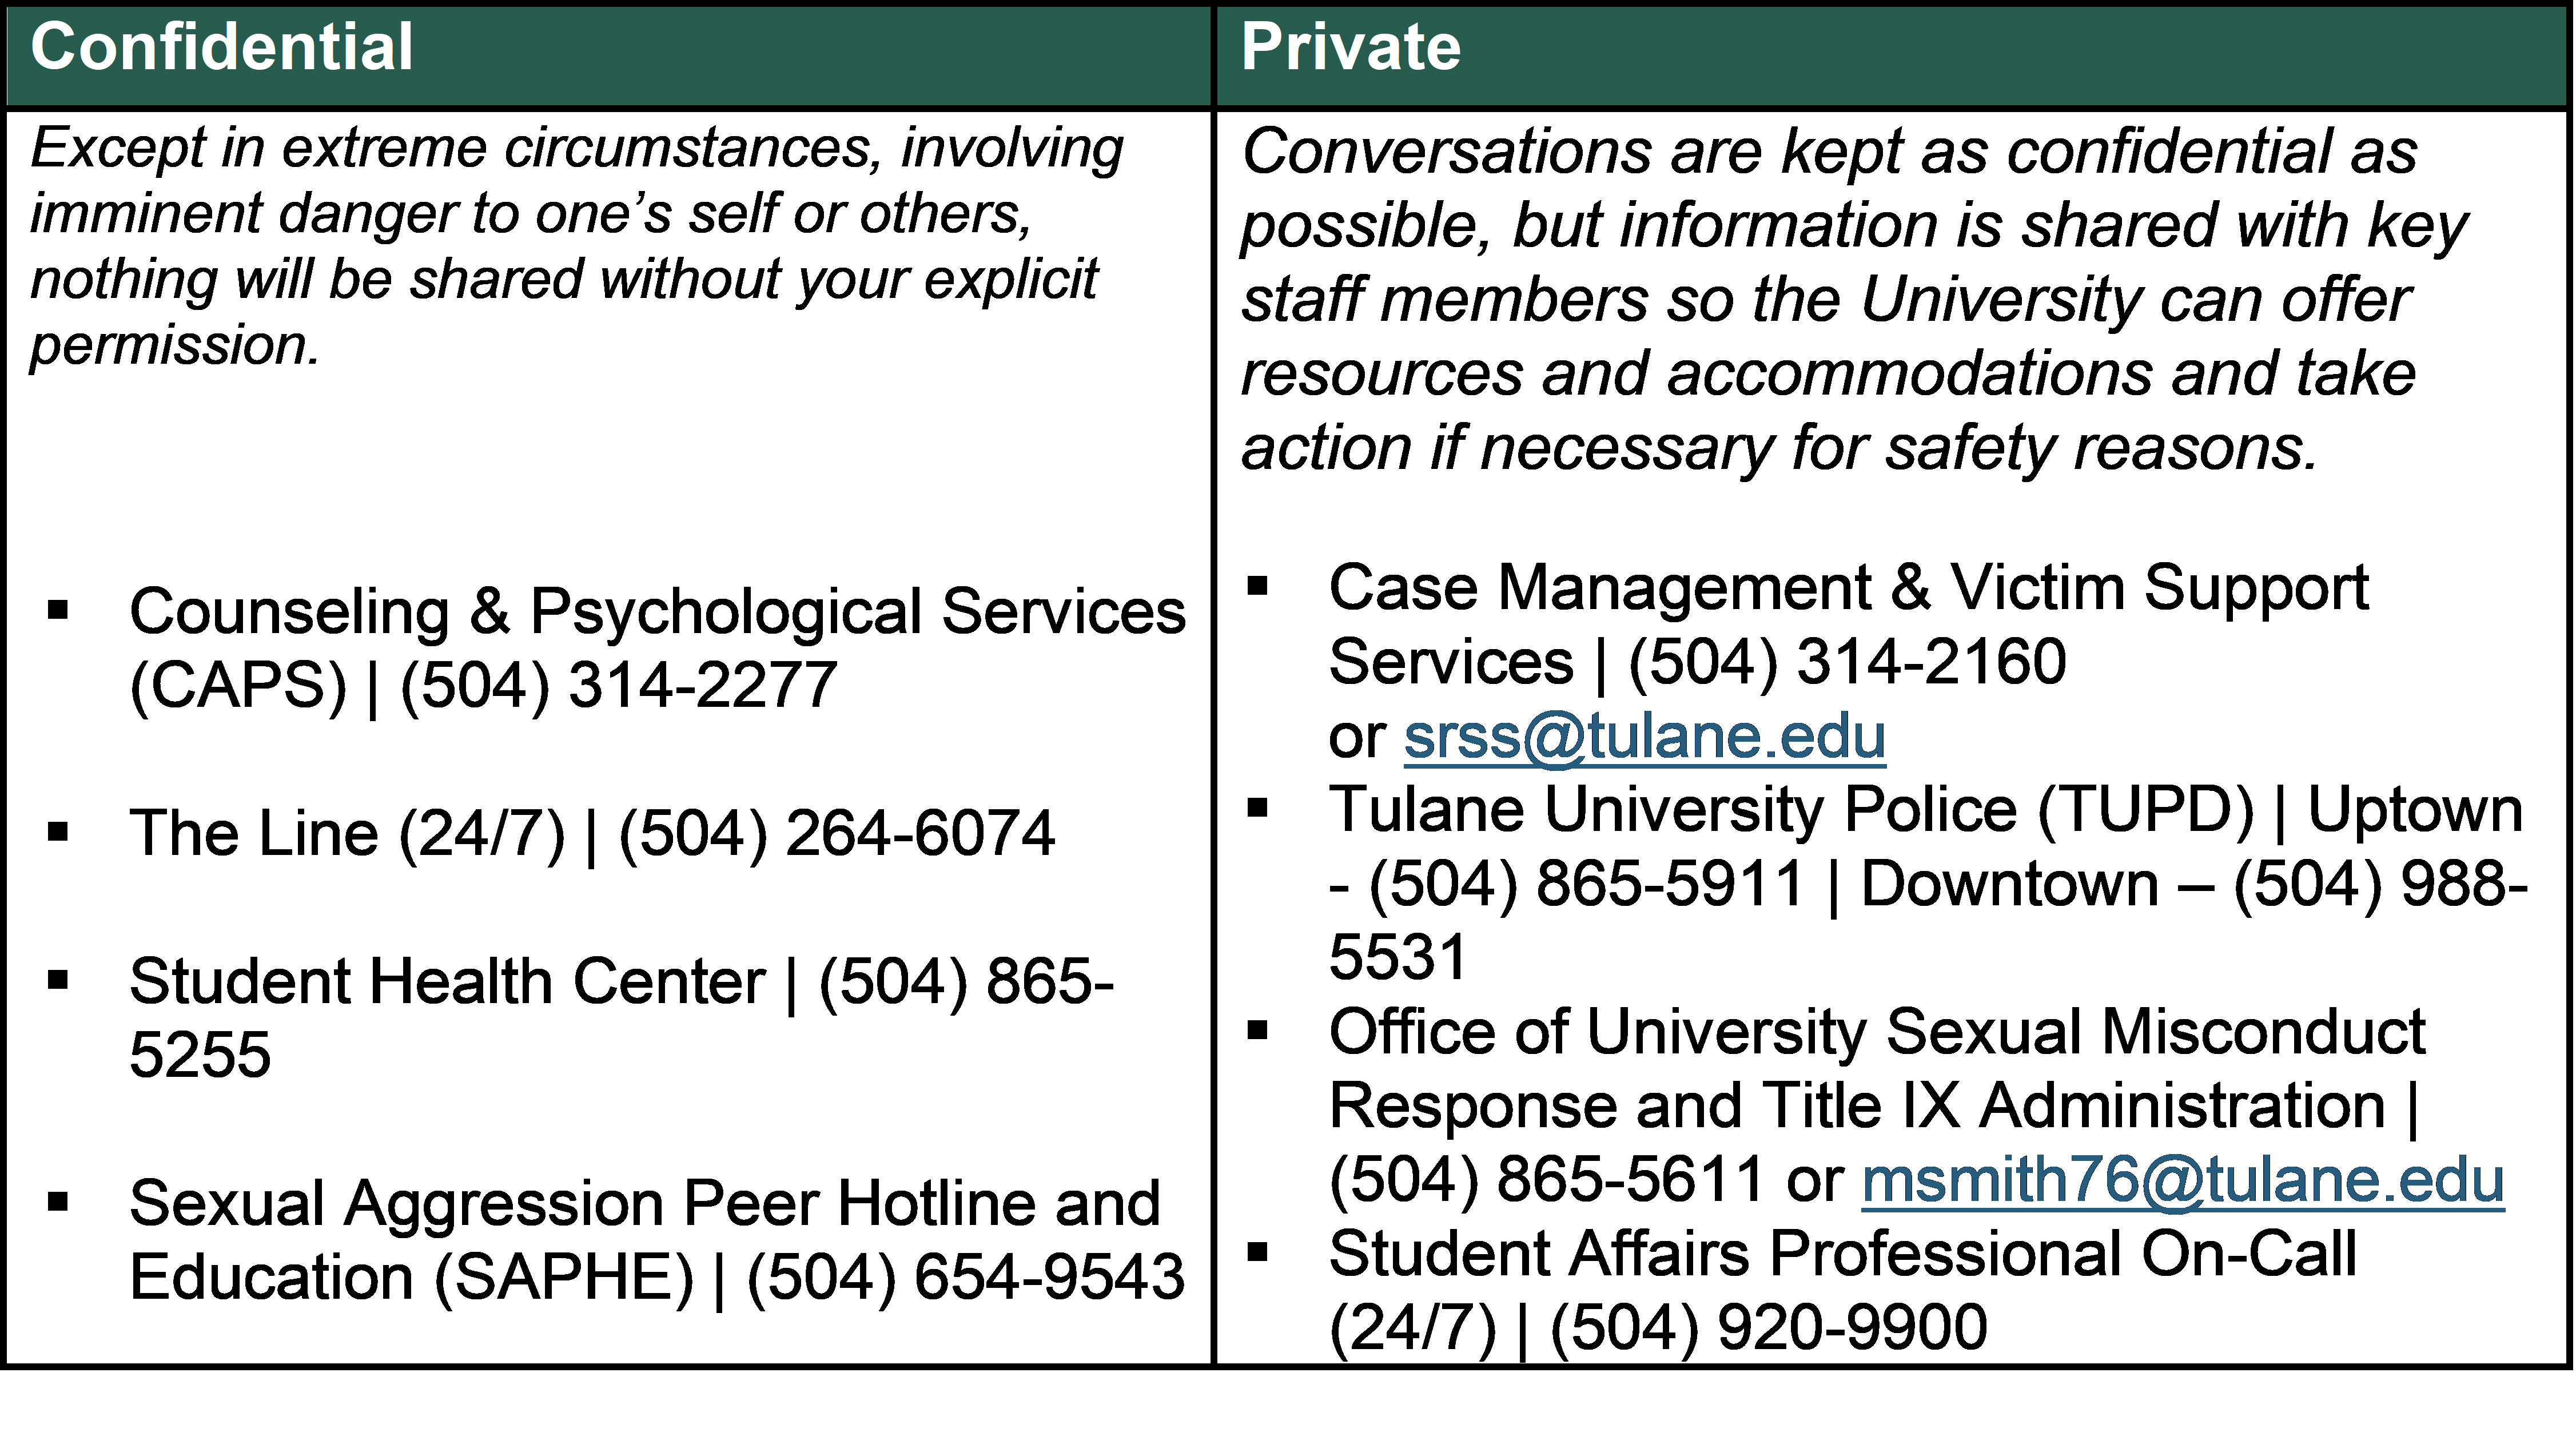
\includegraphics[width=1\linewidth]{figs/title_ix} 
\end{figure}

\newpage

\hypertarget{emergency-preparedness-response}{%
\section{Emergency Preparedness \&
Response}\label{emergency-preparedness-response}}

\begin{figure}

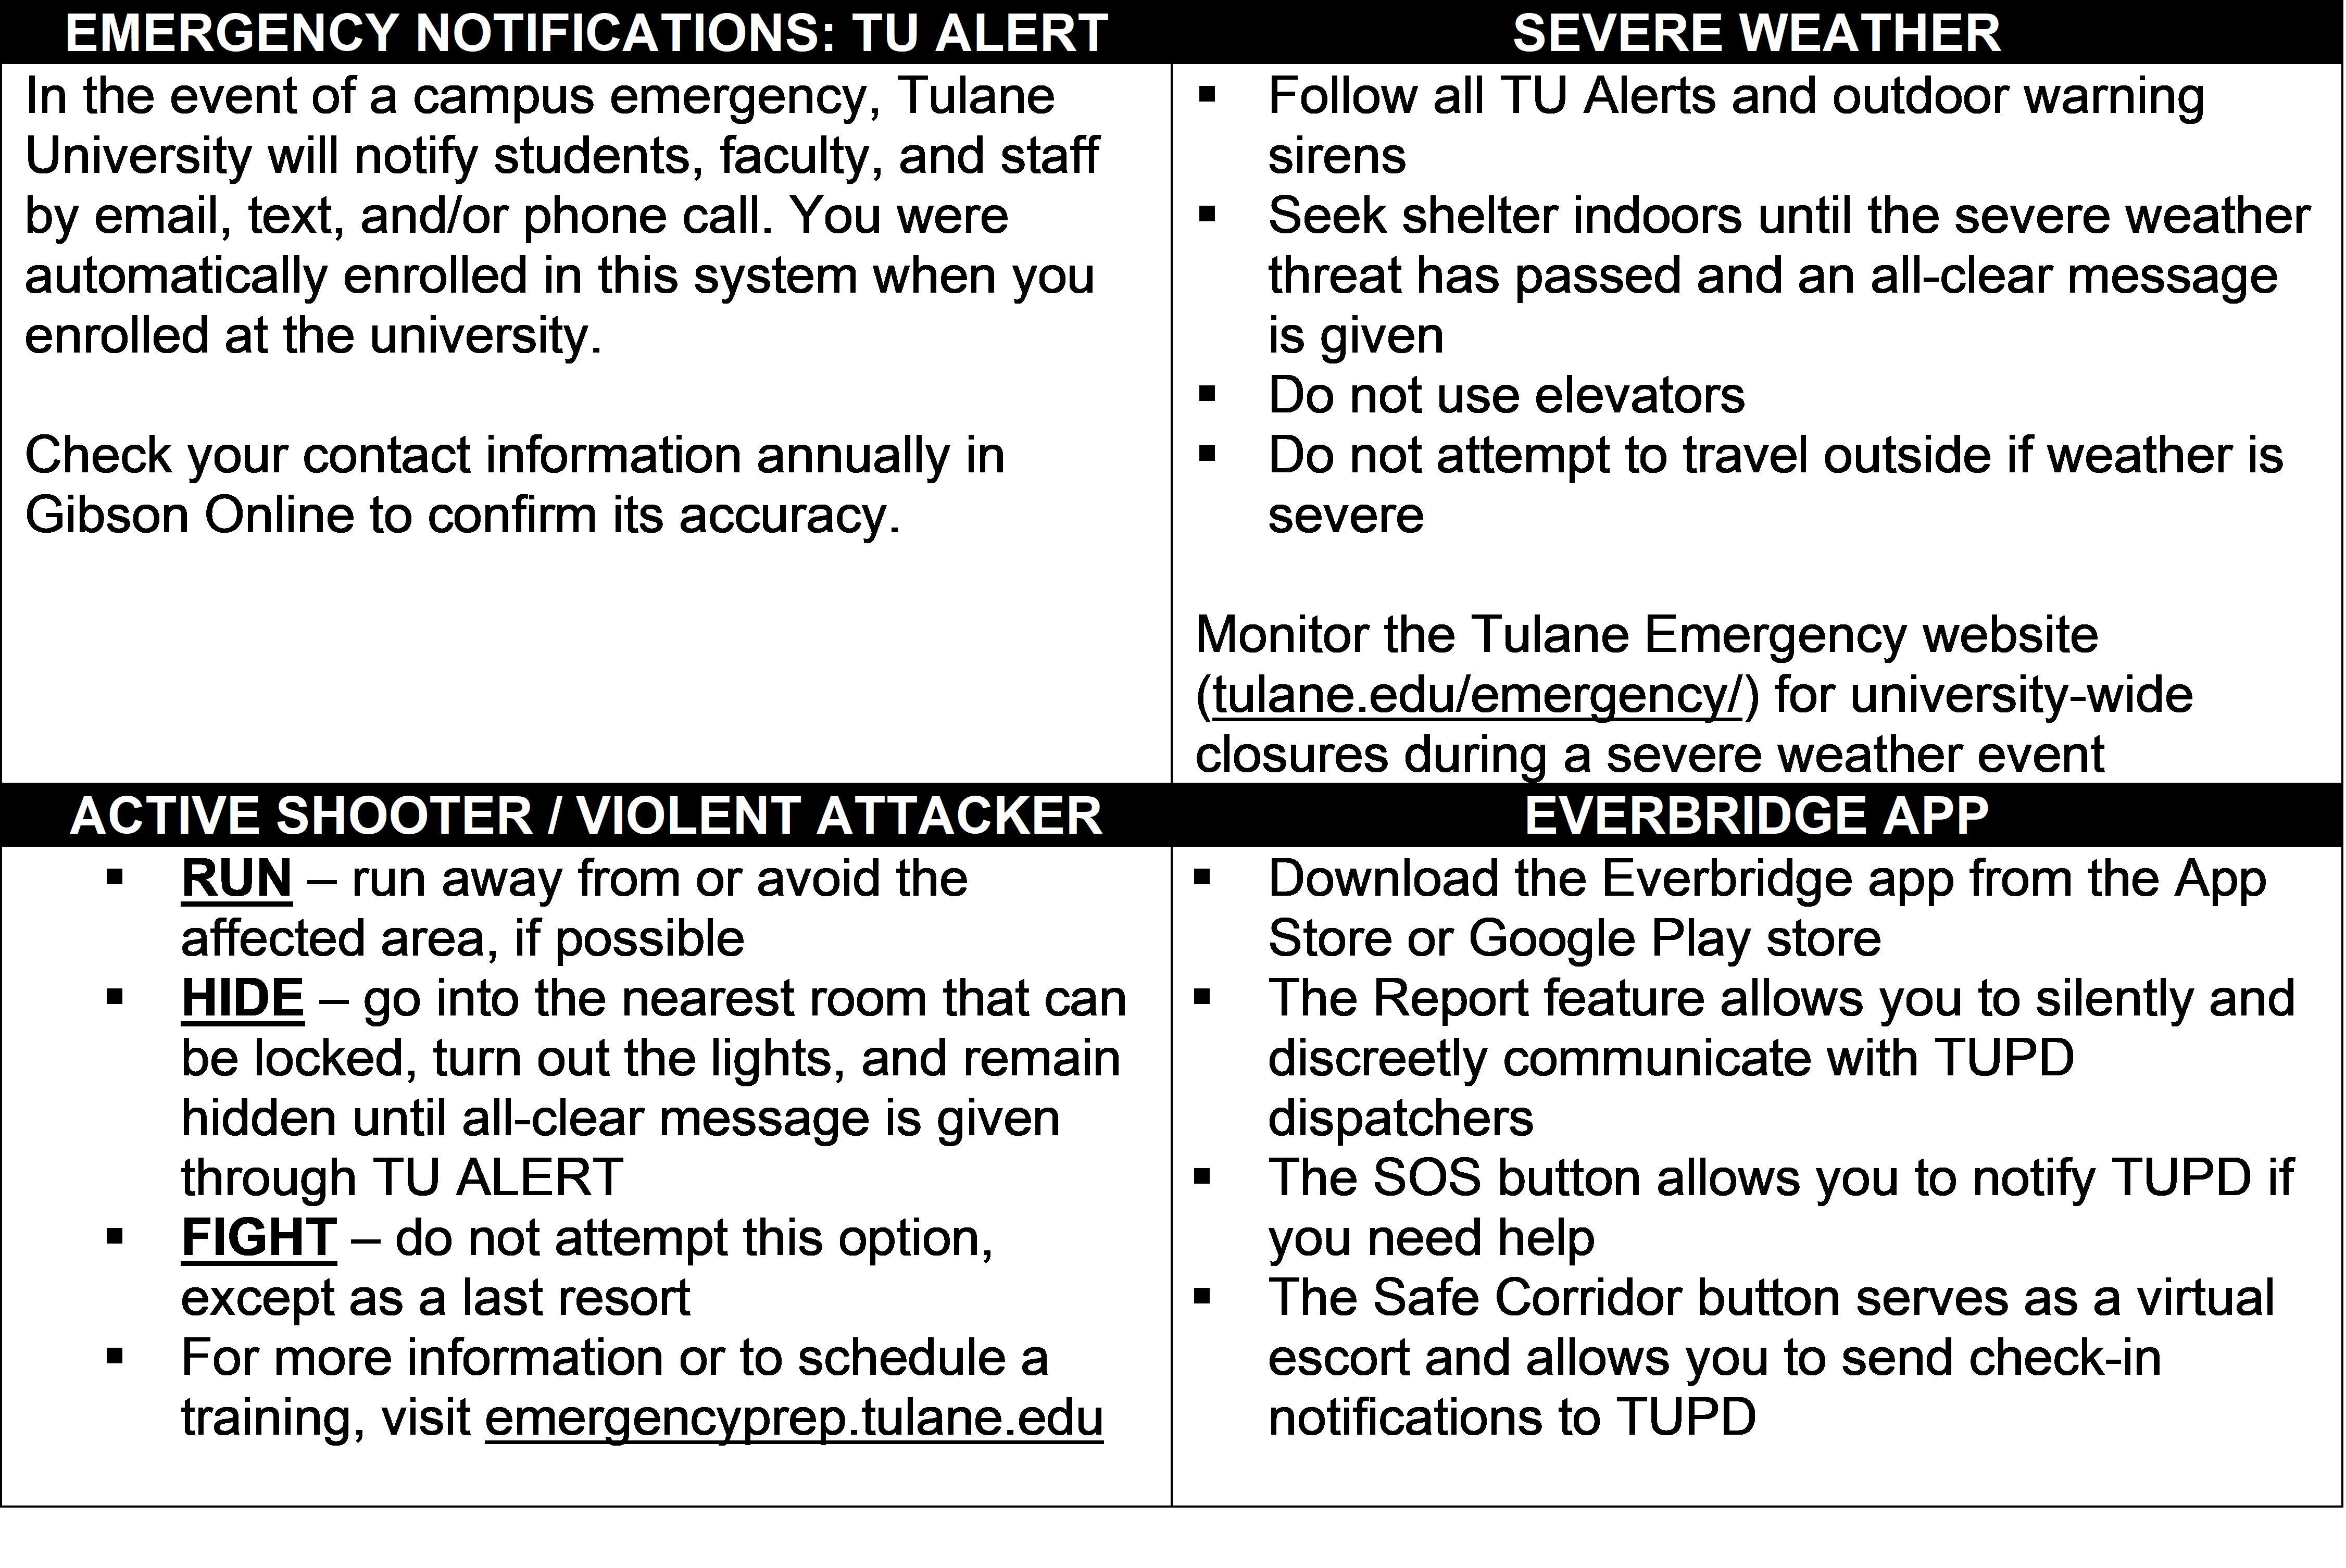
\includegraphics[width=1\linewidth]{figs/emergency} 
\textbf{From: Tulane Office of emergency preparedness and response}
\end{figure}

\end{document}
